\chapter{\textit{Scaffolding}}\label{ch:schaffolding}

Muitas vezes ao nos deparamos com um problema, que precisamos resolver, chagamos a um empasse. Neste o dia a dia, é comum buscarmos ajuda no processo de solução desse problema, mas no âmbito acadêmico (como em processos avaliativos), muitas vezes, isso não é possível. O método de \textit{Scaffolding} surge neste meio, como uma forma de auxiliar o estudante a desenvolver suas habilidades perante uma tarefa a qual ele, sozinho, não tem condição de resolver. 

Podemos definir \textit{Scaffolding} \cite{Belland2017, wood1976} como um “suporte iterativo que faz uso dos conhecimentos do estudante para ajudá-los a participar significativamente e a desenvolver habilidades que estão além de suas capacidades atuais”. Esse tipo de suporte potencializa as habilidades dos estudantes e os ajuda a completar tarefas que, sem o suporte, não poderiam ser resolvidas com os conhecimentos momentâneos do estudante, tais quais resolver o problema central, traçar uma estratégia para o problema, ou mesmo completá-lo. A Figura \ref{fig:scaffoldingInstitucional} exemplifica o processo de funcionamento do método de Scaffolding. 

\begin{figure}[htp]
\begin{center}
\caption{Papel do \textit{Scaffolding} institucional.}
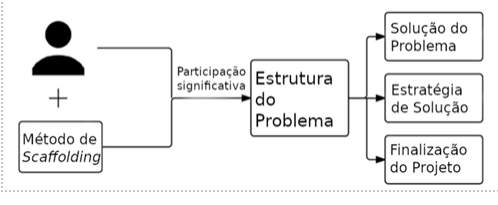
\includegraphics[width=0.8\textwidth]{fig/scaffoldinInstitucional.png}
\label{fig:scaffoldingInstitucional}
\caption*{Fonte: Adaptado de \citeonline{Belland2017}.}
\end{center}
\end{figure}

Entretanto, devemos tomar cuidado ao classificar uma “ajuda” como parte do processo de \textit{Scaffolding}. Isso ocorre, pois, muitas vezes durante o processo de análise dessa ajuda, passamos a chamar de \textit{Scaffolding} toda e qualquer ajuda que auxilie o aluno na resolução do problema. Tal informação é inexata, uma vez que dizer o quê ou como deve ser feito determinada tarefa não pode ser considerada como \textit{Scaffolding}(\cite{Belland2017}, uma vez que esse tipo de abordagem não faz uso nem se constrói a partir do conhecimento prévios do aluno. 

Para que possamos classificar uma ajuda como parte do método de \textit{Scaffolding} é extremamente necessário que a ajuda fornecida faça uso dos conhecimentos prévios do aluno, para que ele possa construir seus novos conhecimentos em cima de seus conhecimentos prévios. Inclusive, o termo \textit{Scaffolding} do inglês significa andaime, uma alusão direta aos andaimes utilizados na construção civil. 

Assim como os andaimes da construção servem de ancoragem para a construção de uma estrutura mais rígida e definitiva, o andaime na educação que estamos chamando de \textit{Scaffolding} serve como ancoragem para a formação de um conhecimento mais sólido sobre o problema a ser trabalhado. E esses “andaimes” podem ser fornecidos por professores, colegas ou, até mesmo, por ferramentas computacionais. 

O método de \textit{Scaffolding} também é composto por três principais elementos: Avaliação Dinâmica, Fornecer a Quantidade Certa de Suporte e Intersubjetividade. Esses três elementos serão descritos a seguir. 

\section{AVALIAÇÃO DINÂMICA}

A avaliação dinâmica está intrinsecamente conectada com a customização do método de \textit{Scaffolding} \cite{Belland2017,wood1976}. A Figura 2 exemplifica a relação entre a avaliação dinâmica e o \textit{Scaffolding}.

\begin{figure}[htp]
\begin{center}
\caption{O papel da Avaliação Dinâmica na Customização do \textit{Scaffolding}.}
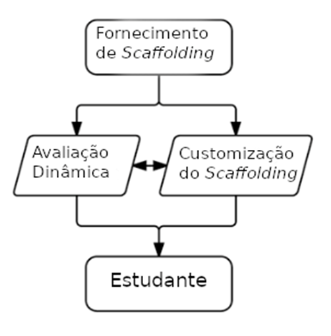
\includegraphics[width=0.7\textwidth]{fig/avaliacaodinamica.png}
\label{fig:avadinamica}
\caption*{Fonte: Adaptado de \citeonline{Belland2017}.}
\end{center}
\end{figure}

A avaliação Dinâmica pode envolver uma série de instruções, onde cada instrução pode ter diferentes níveis de suporte. Então o professor pode determinar, para o atual nível de habilidade do aluno, qual destes suportes é necessário para permitir o desempenho adequado do aluno na tarefa. 

Ao associar a Avaliação Dinâmica com o \textit{Scaffolding}, \citeonline{Belland2017} ressalta que: 

\begin{quoting}[leftmargin=4cm, rightmargin=0cm]
\noindent Avaliação dinâmica pode também ser usada para ajustar o \textit{Scaffolding} que já está sendo fornecido. Neste caso, os professores podem determinar até que ponto a habilidade do aluno está melhorando, de modo a levar ao sucesso sem o uso, ou com menor uso, de \textit{Scaffolding}. E tais ajustes podem ser feitos em tempo real. 
\end{quoting}

\section{FORNECER A QUANTIDADE CERTA DE SUPORTE}

O fornecimento da quantidade certa de suporte se refere a fornecer a suporte ao Scaffolding de acordo com a indicação da avaliação dinâmica \cite{wood1976,Belland2017}. Isso pode ser feito tanto pelo fornecimento de suporte em tempo real \cite{Jadallah2011,vanPol2012,Belland2017}, ou fornecendo a combinação certa de elementos prévios de Scaffolding \cite{Koedinger2006,Belland2017}. Além disso, de acordo com \citeonline[p.18]{Belland2017} e \citeonline[p.17]{wood2003}, providenciar a quantidade correta de suporte depende dos ajustes em uma ou mais das seguintes formas: ajuste das estratégias de suporte que estão sendo utilizadas, as sub-habilidades cujo foco esteja próximo, e o tempo necessário oferecido para o suporte. 

\citeonline{Koedinger2006,Koedinger2007,Belland2017} ressaltam, sobre o ajuste de \textit{Scaffolding}: 

\begin{quoting}[leftmargin=4cm, rightmargin=0cm]
\noindent O ajuste de \textit{Scaffolding} também pode assumir a forma de adicionar diferentes tipos de suporte ou aprimorar o suporte que já estava presente. Isso com base na avaliação dinâmica que indica que os alunos não estão progredindo rápido o suficiente para levar à solução independente da solução de problemas. 
\end{quoting}

Por fim, podemos dizer que, ao fornecer a quantidade certa se suporte ao \textit{Scaffolding}, temos como meta que o aluno não apenas ganhe as habilidades necessárias para realizar a tarefa de forma independente, mas que também assume responsabilidade pela execução da própria tarefa \cite{wood1976,Belland2014, Belland2017}. Em outras palavras, estamos dizendo que queremos que o aluno não apenas desenvolva suas capacidades, mas também tenha mais vontade de resolver tarefas complexas de forma independente \cite{Belland2013, Belland2017}. 

\section{INTERSUBJETIVIDADE}

A intersubjetividade é crucial para a definição de \textit{Scaffolding} e para a ideia de transferir responsabilidades para o aluno. Segundo a intersubjetividade, os alunos precisam ser capazes de reconhecer uma solução apropriada para problemas semelhantes, antes de serem capazes de executar a mesma tarefa de forma independente \cite{wood1976,Mortimer2009,Mahardale2014,Belland2017}. De acordo com \citeonline[p.16]{Belland2017}, sem a intersubjetividade os alunos são considerados incapazes de se engajar no desempenho independente da habilidade alvo apresentado na Figura \ref{fig:intersubjetividade}. 

\begin{figure}[htp]
\begin{center}
\caption{Exposição da Intersubjetividade e Engajamento no \textit{Scaffolding}.}
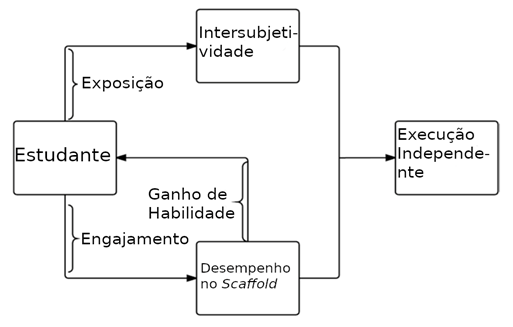
\includegraphics[width=0.7\textwidth]{fig/intersubjetividade.png}
\label{fig:intersubjetividade}
\caption*{Fonte: Adaptado de \citeonline{Belland2017}.}
\end{center}
\end{figure}

De acordo com \citeonline[p.22]{Belland2017} e \citeonline{wertsch2005}, a intersubjetividade pode ser alcançada sem o conhecimento de como executar a habilidade que o \textit{Scaffolding} se destina a desenvolver. Para \citeonline[p.21]{Belland2017} e \citeonline{Rogoff1997}, é importante que notemos que não é necessário existir um mesmo entendimento entre aluno e professor.  Isso ocorre, pois, parceiros em uma mesma atividade possuem perspectiva diferentes, o que pode moldar o entendimento da tarefa. Além disso, para \citeonline[p.22]{Belland2017} e \cite{wertsch1985zone}, se uma criança e um adulto tivessem uma compreensão idêntica de qual seria a solução mais apropriada para um problema semelhante ao que está sendo abordado, então pode ser criança não precise de \textit{Scaffolding}. 

\section{FORMAS DE SCAFFOLDING}

Podemos classificar, segundo \citeonline[p.22]{Belland2017}, três formas de trabalhar com o método de Scaffolding. Essas formas podem ser separadas em: \textit{Scaffolding} Um a Um (SUU), \textit{Scaffolding} por Pares (SPP) e \textit{Scaffolding} Baseado em Computadores (SBC). 

A Tabela \ref{tab:tipsScaf} exemplifica a comparação entre as três formas de \textit{Scaffolding}. As três formas de \textit{Scaffolding} serão descritas na sequência do trabalho. 

\begin{comment}
\setlength{\tabcolsep}{1.505625pt}
\renewcommand{\arraystretch}{1.2}
\begin{table}[ht]
\captionof{table}{Visão Geral dos tipos de \textit{Scaffolding}.}
\label{tab:tipsScaf}
\begin{tabular}{|l|l|l|l|}
\hline
\multicolumn{1}{|p{82.80937pt}}{} & \multicolumn{1}{|p{114.4275pt}}{\centering {\bfseries \textit{Scaffolding} Um a Um }} & \multicolumn{1}{|p{112.921875pt}}{\centering {\bfseries \textit{Scaffolding} Baseado em Computador }} & \multicolumn{1}{|p{113.67469pt}|}{\centering {\bfseries \textit{Scaffolding} por Pares }}\\ \hline

\multicolumn{1}{|p{82.80937pt}}{\centering {\bfseries O que \'e? }} & \multicolumn{1}{|p{114.4275pt}}{\centering Professor trabalhando individualmente com um estudante } & \multicolumn{1}{|p{112.921875pt}}{\centering Fun\c{c}\~ao do \textit{Scaffolding} cumprida por uma ferramenta computacional que pode ser incorporada no curr\'{\i}culo ou uma ferramenta que os estudantes usem quando se engajam em um problema fora do sistema } & \multicolumn{1}{|p{113.67469pt}|}{\centering \textit{Scaffolding} promovido por pares com habilidades superiores ou de mesmo n\'{\i}vel }\\ 
\hline 
\multicolumn{1}{|p{82.80937pt}}{\centering {\bfseries Entre as formas de \textit{Scaffolding}, quais suas vantagens relativas? }} & \multicolumn{1}{|p{114.4275pt}}{\centering Leva \`a influ\^encia mais forte nos resultados de aprendizagem \\ 
\strut\ \\ 
\'E o melhor para a customiza\c{c}\~ao din\^amica } & \multicolumn{1}{|p{112.921875pt}}{\centering \'E o mais utiliz\'avel \\ 
\strut\ \\ 
Tem paci\^encia infinita } & \multicolumn{1}{|p{113.67469pt}|}{\centering \'E a forma mais utiliz\'avel de \textit{Scaffolding} que envolve intera\c{c}\~oes individuais }\\ 
\hline 
\multicolumn{1}{|p{82.80937pt}}{\centering {\bfseries Entre as formas de \textit{Scaffolding}, quais suas desvantagens relativas? }} & \multicolumn{1}{|p{114.4275pt}}{\centering Menos utiliz\'avel } & \multicolumn{1}{|p{112.921875pt}}{\centering Menos din\^amico } & \multicolumn{1}{|p{113.67469pt}|}{\centering Provedor de Scaffolding n\~ao \'e, necessariamente, mais h\'abil }\\ 
\hline 
\end{tabular}
\caption*{Fonte: Construção do Autor.}
\end{table}
\end{comment}


\begin{table}[ht]
\caption{Visão Geral dos tipos de \textit{Scaffolding}.}
\label{tab:tipsScaf}
\begin{tabular}{p{82.80937pt}|p{114.4275pt}|p{112.921875pt}|p{113.67469pt}}
\hline
\textbf{} & \textbf{\textit{Scaffolding} Um a Um} & \textbf{\textit{Scaffolding} Baseado em Computador} & \textbf{\textit{Scaffolding} por Pares}\\ 
\hline
\textbf{O que é?} & Professor trabalhando individualmente com um estudante & Função do \textit{Scaffolding} cumprida por uma ferramenta computacional que pode ser incorporada no currículo ou uma ferramenta que os estudantes usem quando se engajam em um problema fora do sistema & \textit{Scaffolding} promovido por pares com habilidades superiores ou de mesmo nível\\ 
\hline
\textbf{Entre as formas de \textit{Scaffolding}, quais suas vantagens relativas?} & Leva à influência mais forte nos resultados de aprendizagem & É o mais utilizável & Tem paciência infinita\\ 
\hline
\textbf{Entre as formas de \textit{Scaffolding}, quais suas desvantagens relativas?} & Menos utilizável & Menos dinâmico & Provedor de Scaffolding não é, necessariamente, mais habil\\ 
\hline
\end{tabular}
\caption*{Fonte: Construção do Autor.}
\end{table}

\subsection{\textit{Scaffolding} Um a Um}

\citeonline[p.21]{Belland2017} define o SUU como sendo um professor trabalhando individualmente com um estudante para avaliar dinamicamente o nível atual do estudante, provendo a quantidade correta de suporte para que o estudante para que ele ganhe a habilidade na tarefa em questão. Além de personalizar o suporte conforme necessário até que o \textit{Scaffolding} possa ser completamente retirado e o estudante possa executar a tarefa de forma independente \cite{Chi1996,Graesser1997,Lepper1997,vanPol2010,Belland2014}.
 
A utilização do Scaffolding Um a Um é útil ao pensarmos nas intenções do método de Scaffolding, seja na utilização pelo professor, nos meios utilizados, e nas estratégias específicas utilizadas \cite{vanPol2010,Belland2012,Belland2017}. As intenções do SUU incluem o recrutamento, estruturação das tarefas, manutenção da direção, redução dos graus de liberdade e controle de frustração \cite{vanPol2010,Belland2017}.

De acordo com \citeonline[p.27]{Belland2017}, as formas de utilização do SUU incluem modelar, questionar, explicar, dar dicas e providenciar um \textit{feedback} \cite{vanPol2010}. \citeonline[p.22]{Belland2017} e \citeonline{Lin2014} dizem que: 

\begin{quoting}[leftmargin=4cm, rightmargin=0cm]
\noindent Para promover a consideração das relações entre as diferentes individualidades envolvidas em um problema, o professor pode levar os alunos a considerar tais relações e ilustrar como fazê-lo. 
\end{quoting}

\citeonline[p.23]{Belland2017} conclui dizendo que, devido a forma altamente contagiante de sua estrutura, o SUU é geralmente considerado como sendo a forma ideal de \textit{Scaffolding} \cite{Chi1996,Graesser1997,Belland2015}. Entre todas as formas de \textit{Scaffolding} , \citeonline[p.24]{Belland2014} diz que SUU tende a levar aos melhores resultados, conforme indica o trabalho de \citeonline[p.1]{vanLehn2011}.  
\subsection{\textit{Scaffolding} Por Pares }

\textit{Scaffolding}por pares se refere ao fornecimento de suporte por pares de mesma idade ou conhecimento similar e exalta a força do número de pares em salas de aula \cite{Pata2006,Davin2013,Sabet2013,Belland2017}. Porém, o SPP pode também envolver crianças mais velhas que dão suporte a crianças mais jovens, com o uso de seus conhecimentos sobre a tarefa em questão. 

\citeonline[p.21]{Belland2014} e  \citeonline[p.25]{Belland2017}, sugere que o SPP necessita o fornecimento de uma estrutura que oriente o desenvolvimento do suporte provido por \textit{Scaffolding}. Onde essa estrutura pode guiar o fornecedor desse suporte com a forma e o momento de uso de estratégias de \textit{Scaffolding}.

Para finalizar, \citeonline[p.21]{Belland2014} e  \citeonline[p.25]{Belland2017}, conclui que: 

\begin{quoting}[leftmargin=4cm, rightmargin=0cm]
\noindent É improvável que \textit{Scaffolding} por pares seja suficiente como forma única de suporte por \textit{Scaffolding}, uma vez que os pares com capacidades semelhantes não têm conteúdo ou a experiência pedagógica necessária para se envolverem na avaliação dinâmica e na personalização que é característica do \textit{Scaffolding} por Pares. 
\end{quoting}
\subsection{\textit{Scaffolding} Baseado em Computador}

De acordo com \citeonline[p.1]{Belland2017}, \textit{Scaffolding} baseado em computador auxilia os estudantes a se engajarem e adquirirem habilidades em tarefas que estão além de suas habilidades não assistidas \cite{Hannafin1999,Quintana2004,Belland2014}. Especificamente, o SBC ajuda os estudantes na geração de soluções para problemas complexos e mal estruturados, e é fornecido inteiramente por uma ferramenta baseada em computador \cite{Belland2017}.

Isso significa que uma ferramenta computacional é capaz de ampliar a capacidade dos alunos de forma que eles se tornam capazes de realizar tarefas que estão em um nível mais alto que suas capacidades atuais não assistidas. \citeonline[p.21]{Belland2017} afirma que “\textit{Scaffolding} baseado em computador tem tido um tamanho de efeito muito substancial em pesquisas anteriores, em comparação com intervenções semelhantes, e isso merece mais pesquisas metodologia”. 